
%\cprotEnv\begin{question}
%The Dow-Jones Industrial Average (DJIA) was first introduced by Charles Dow in 1896 and has since become one of the main references for stock market performance on the New York Stock Exchange.
%
%In this post, we will use it to better understand the pros and cons of simple Linear Regression models, the assumptions they rely on, and how we can use them for feature selection.
%
%Its value is determined with a weighted average of 30 stock prices. Since the Dow components change over time, using the provided dataset (\href{"https://github.com/matteosan1/finance_course/raw/master/input_files/dji.csv}{dji.csv}) and a list of 35 assets, determine which of them are included in the calculation given a time interval. Try to interpret the results.
%
%\textbf{Hint}: in order to cross-check your result split the dataset in two parts (before and after August 2020), then fit the model with the first part and test it with the second.
%\begin{ipython}
%selected = ['AAPL', 'AMGN', 'AXP', 'BA', 'CAT', 'CRM', 'CSCO', 'CVX', 'DD', 'DIS', 
%            'DOW', 'GE', 'GS', 'HD', 'HON', 'IBM', 'INTC', 'JNJ', 'JPM', 'KO', 'MCD', 
%            'MMM', 'MRK', 'MSFT', 'NKE', 'PFE', 'PG', 'RTX', 'TRV', 'UNH', 'V', 'VZ', 
%            'WBA', 'WMT', 'XOM']
%\end{ipython}
%\end{question}
%
%\cprotEnv\begin{solution}
%Load the dataset and split into two dataframes DJI and the other tickers.
%\begin{ipython}
%import pandas as pd
%
%closing = pd.read_csv("dji.csv", index_col='Date')
%DJI = closing['DJI'].copy()
%closing.drop(columns='DJI', inplace=True)
%\end{ipython} 
%	
%\begin{figure}[htbp]
%\centering
%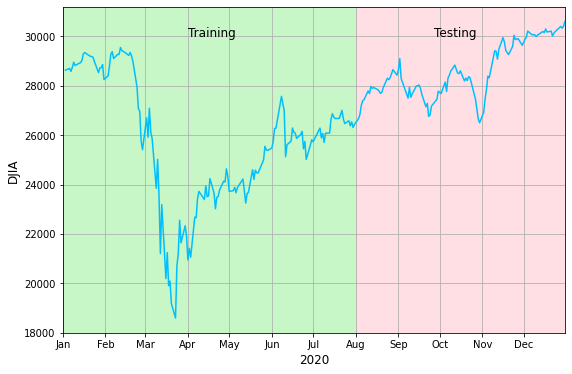
\includegraphics[width=0.7\textwidth]{figures/dji}
%\caption{DJIA index daily values in 2020. The dataset has been divided into two parts for training and testing purpose.}
%\label{fig:dji-returns}
%\end{figure}
%	
%We need to fit the linear model to the available data prior to August 2020 (\emph{notice that the dataset already contains the intercept column to take care of the $\alpha$ parameter}), see Fig.~/ref{fig:dji-returns}.
%\begin{ipython}
%import statsmodels.api as sm
%
%model = sm.OLS(DJI[DJI.index <='2020-07-31'], 
%               closing[closing.index <='2020-07-31']).fit()
%print (model.summary())
%\end{ipython}
%\begin{ioutput}
%                          OLS Regression Results                            
%==============================================================================
%Dep. Variable:                    DJI   R-squared:                       1.000
%Model:                            OLS   Adj. R-squared:                  1.000
%Method:                 Least Squares   F-statistic:                 2.107e+06
%Date:                Tue, 08 Nov 2022   Prob (F-statistic):          1.99e-297
%Time:                        18:16:13   Log-Likelihood:                -364.32
%No. Observations:                 143   AIC:                             800.6
%Df Residuals:                     107   BIC:                             907.3
%Df Model:                          35                                         
%Covariance Type:            nonrobust                                         
%==============================================================================
%coef    std err          t      P>|t|      [0.025      0.975]
%------------------------------------------------------------------------------
%AAPL          28.1315      0.238    118.405      0.000      27.660      28.602
%AMGN           0.0701      0.098      0.714      0.477      -0.124       0.265
%AXP            6.2508      0.261     23.940      0.000       5.733       6.768
%BA             7.0296      0.047    149.349      0.000       6.936       7.123
%CAT            6.8530      0.160     42.953      0.000       6.537       7.169
%CRM            0.0452      0.123      0.367      0.714      -0.199       0.289
%CSCO           6.9258      0.564     12.274      0.000       5.807       8.044
%CVX            7.6117      0.260     29.233      0.000       7.096       8.128
%DD             0.4722      0.318      1.484      0.141      -0.159       1.103
%DIS            6.9450      0.178     39.057      0.000       6.593       7.298
%DOW            6.3940      0.387     16.541      0.000       5.628       7.160
%GE             0.2437      0.216      1.130      0.261      -0.184       0.671
%GS             6.9331      0.122     56.636      0.000       6.690       7.176
%HD             6.6309      0.096     69.009      0.000       6.440       6.821
%HON           -0.3708      0.193     -1.918      0.058      -0.754       0.012
%IBM            7.3397      0.202     36.317      0.000       6.939       7.740
%INTC           6.5288      0.199     32.789      0.000       6.134       6.924
%JNJ            6.7114      0.240     27.962      0.000       6.236       7.187
%JPM            6.7418      0.236     28.578      0.000       6.274       7.209
%KO             6.9641      0.572     12.173      0.000       5.830       8.098
%MCD            6.8349      0.150     45.446      0.000       6.537       7.133
%MMM            6.4935      0.146     44.401      0.000       6.204       6.783
%MRK            7.5556      0.318     23.792      0.000       6.926       8.185
%MSFT           6.4336      0.155     41.509      0.000       6.126       6.741
%NKE            6.7713      0.231     29.369      0.000       6.314       7.228
%PFE            8.0045      0.466     17.163      0.000       7.080       8.929
%PG             7.0308      0.294     23.894      0.000       6.447       7.614
%RTX            8.4790      0.301     28.136      0.000       7.882       9.076
%TRV            6.7275      0.194     34.767      0.000       6.344       7.111
%UNH            6.7560      0.073     93.183      0.000       6.612       6.900
%V              7.2610      0.174     41.824      0.000       6.917       7.605
%VZ             6.6514      0.631     10.546      0.000       5.401       7.902
%WBA            6.2044      0.331     18.750      0.000       5.548       6.860
%WMT            6.7940      0.211     32.258      0.000       6.376       7.212
%XOM            6.0549      0.487     12.435      0.000       5.090       7.020
%intercept     -4.1082     21.263     -0.193      0.847     -46.259      38.043
%==============================================================================
%Omnibus:                       19.720   Durbin-Watson:                   2.012
%Prob(Omnibus):                  0.000   Jarque-Bera (JB):               62.557
%Skew:                          -0.398   Prob(JB):                     2.61e-14
%Kurtosis:                       6.141   Cond. No.                     5.70e+04
%==============================================================================
%\end{ioutput}
%
%From the $p$-values in Figure~\ref{fig:p-values} (left), we can quickly identify the stocks whose weights are not meaningfully different from zero, namely: AMGN, CRM, DD, GE, and HON. The reason is simply that they are not part of the DJIA in the considered period.
%Repeating the fit with the updated model shows that all the included tickers are still contributing to the DJIA index determination, see Fig.~\ref{fig:p-values} (right).
%	
%\begin{ipython}
%selected_columns = list(model.pvalues[model.pvalues<0.05].index)
%
%model_small = sm.OLS(DJI[DJI.index <= '2020-07-31'], 
%                     closing[selected_columns][closing.index <= '2020-07-31']).fit()
%print (model_small.summary())
%\end{ipython}
%\begin{ioutput}
%                        OLS Regression Results                                
%==============================================================================
%Dep. Variable:                    DJI   R-squared (uncentered):          1.000
%Model:                            OLS   Adj. R-squared (uncentered):     1.000
%Method:                 Least Squares   F-statistic:                 2.434e+08
%Date:                Thu, 26 Jan 2023   Prob (F-statistic):               0.00
%Time:                        11:59:44   Log-Likelihood:                -369.56
%No. Observations:                 143   AIC:                             799.1
%Df Residuals:                     113   BIC:                             888.0
%Df Model:                          30                                                  
%Covariance Type:            nonrobust                                                  
%==============================================================================
%                 coef    std err          t      P>|t|      [0.025      0.975]
%------------------------------------------------------------------------------
%AAPL          28.1695      0.229    123.120      0.000      27.716      28.623
%AXP            6.2176      0.250     24.878      0.000       5.722       6.713
%BA             7.0379      0.045    157.710      0.000       6.949       7.126
%CAT            6.7754      0.133     50.871      0.000       6.511       7.039
%CSCO           7.2883      0.535     13.620      0.000       6.228       8.348
%CVX            7.5201      0.239     31.522      0.000       7.047       7.993
%DIS            6.8027      0.163     41.760      0.000       6.480       7.125
%DOW            6.6917      0.338     19.793      0.000       6.022       7.361
%GS             6.9423      0.116     59.693      0.000       6.712       7.173
%HD             6.6851      0.089     75.149      0.000       6.509       6.861
%IBM            7.2860      0.196     37.126      0.000       6.897       7.675
%INTC           6.4310      0.189     34.007      0.000       6.056       6.806
%JNJ            6.7935      0.215     31.583      0.000       6.367       7.220
%JPM            6.8400      0.214     31.945      0.000       6.416       7.264
%KO             6.5188      0.494     13.206      0.000       5.541       7.497
%MCD            6.7657      0.139     48.518      0.000       6.489       7.042
%MMM            6.4385      0.121     53.174      0.000       6.199       6.678
%MRK            7.5965      0.296     25.622      0.000       7.009       8.184
%MSFT           6.5577      0.134     48.935      0.000       6.292       6.823
%NKE            6.7307      0.208     32.385      0.000       6.319       7.142
%PFE            8.0817      0.454     17.806      0.000       7.182       8.981
%PG             6.9862      0.267     26.144      0.000       6.457       7.516
%RTX            8.6628      0.275     31.476      0.000       8.118       9.208
%TRV            6.5894      0.181     36.417      0.000       6.231       6.948
%UNH            6.6966      0.066    100.982      0.000       6.565       6.828
%V              7.2778      0.160     45.487      0.000       6.961       7.595
%VZ             6.3851      0.526     12.134      0.000       5.343       7.428
%WBA            6.2725      0.304     20.631      0.000       5.670       6.875
%WMT            6.9055      0.198     34.832      0.000       6.513       7.298
%XOM            6.5498      0.443     14.782      0.000       5.672       7.428
%==============================================================================
%Omnibus:                       27.413   Durbin-Watson:                   1.905
%Prob(Omnibus):                  0.000   Jarque-Bera (JB):               91.998
%Skew:                          -0.630   Prob(JB):                     1.05e-20
%Kurtosis:                       6.722   Cond. No.                     1.70e+03
%==============================================================================
%\end{ioutput}
%\begin{figure}[htbp]
%\centering
%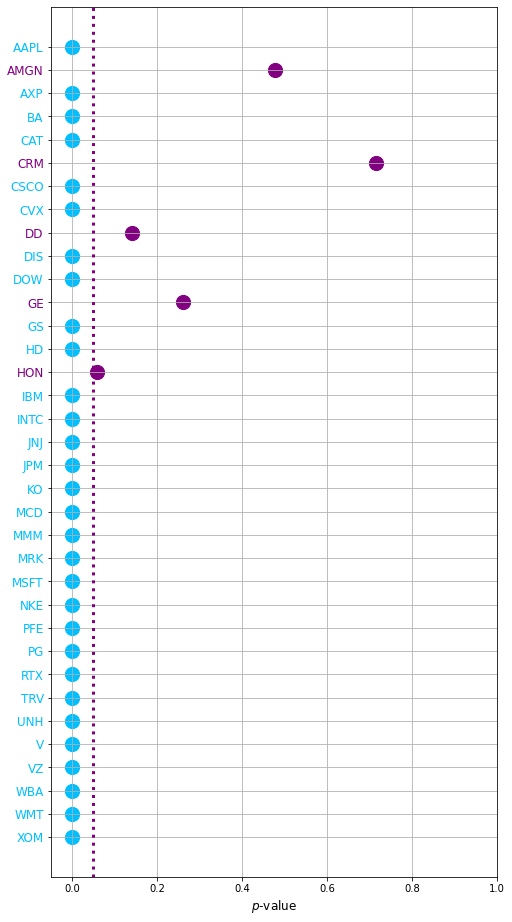
\includegraphics[width=0.4\textwidth]{figures/p-values}
%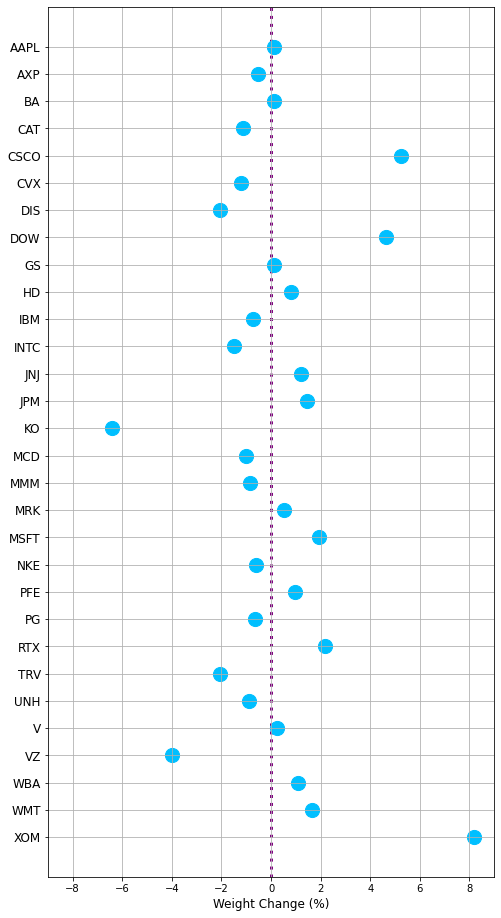
\includegraphics[width=0.4\textwidth]{figures/delta_weights}
%\caption{$p$-values resulting from the linear model fit to DJIA returns (left). Parameter percentage difference according to the two models described in the text (right).}
%\label{fig:p-values}
%\end{figure}
%	
%Now that we have a good model it is possible to check how it behaves on the test sample (i.e. from August to December 2020). The result is shown in Figure~\ref{fig:prediction}. The residuals plot, the difference between predicted and actual values of the DJIA, shows that there is a clear degradation of the performance after September, see Fig.~\ref{fig:residuals}.
%
%\begin{ipython}
%residuals = DJI-model_small.predict(closing[selected_columns])
%\end{ipython}
%	
%\begin{figure}[htbp]
%\centering
%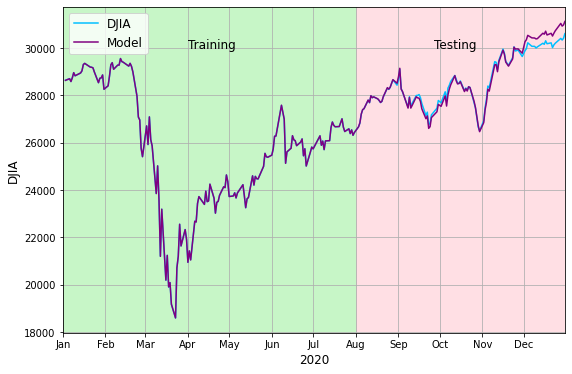
\includegraphics[width=0.7\textwidth]{figures/prediction}
%\caption{Model prediction to DJIA index performance comparison.}
%\label{fig:prediction}
%\end{figure}
%
%As we can see, our model works extremely well for the first few weeks of the testing period and then it completely falls apart. The reason for this puzzling behavior is surprisingly simple: the fundamental assumption underlying our model was no longer valid. The \textbf{composition of the DJIA changed on Aug 31st, 2020} with Pfizer, Raytheon, and Exxon Mobile being dropped and replaced by Amgen, Honeywell, and Salesforce.
%
%\begin{figure}[htbp]
%\centering
%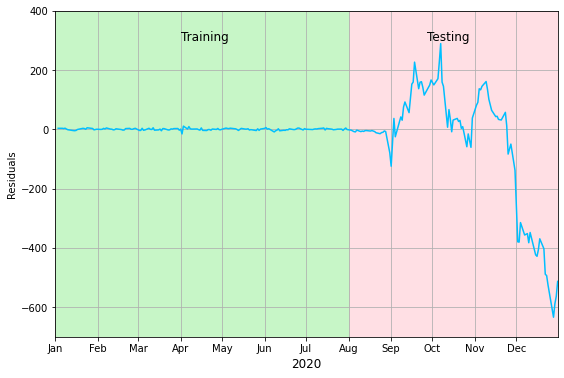
\includegraphics[width=0.7\textwidth]{figures/residuals}
%\caption{Residuals of the linear model.}
%\label{fig:residuals}
%\end{figure}
%\end{solution}

\begin{question}
Stock A has a $\beta$ of 1.2 and Stock B has a $\beta$ of 0.6. Which of the following statements is true? 
\begin{enumerate}[label=\emph{\alph*})]
\tightlist
\item Stock A has more unsystematic risk than Stock B;
\item Stock B has more systematic risk than Stock A; 
\item if the risk-free rate and the market risk premium are both positive, Stock A has a higher expected return than Stock B according to the CAPM;
\item both \emph{a} and \emph{b} are true;
\item both \emph{b} and \emph{c} are true
\end{enumerate}
\end{question}

\begin{solution}
The correct answer is \emph{c} indeed according to CAPM formula
\[r_i = r_f + \beta_i (r_M - r_f)\]
if both $r_f$ and $(r_M - r_f)$ are positive then $r_A > r_B$.
\end{solution}	

\begin{question}
Consider a stock with a $\beta$ of 1.5. Which of the following statements is true?

\begin{enumerate}[label=\emph{\alph*}]
\tightlist
\item when the market goes down by 1.5\%, on average, the stock goes down by 1\%;
\item when the market goes up by 1.5\%, on average, the stock goes up by 1\%;
\item when the market goes up by 1\%, on average, the stock goes down by 1.5\%;
\item when the market goes down by 1\%, on average, the stock goes down by 1.5\%. 
\item both \emph{a} and \emph{b}.	
\end{enumerate}
\end{question}

\begin{solution}
The correct answer is \emph{d} since $\beta$ measures the slope of the regression line of the expected return of the stock vs the expected return of the market. So by definition it represents the variation of the stock expected return given the a unit variation of the expected return of the market.
\end{solution}	

\begin{question}
Suppose that the risk-free rate is 3\% and the market risk premium is 8\%. According to the CAPM, what is the required rate of return on a stock with a $\beta$ of 2 ?
\end{question}

\begin{solution}
Careful! The market risk premium is 8\%. This means that $r_M - r_f  = 8\%$. Plug this into the CAPM equation to get

\begin{equation*}
r = r_f + \beta(r_M - r_f) = 3\% + 2\cdot(8\%) =19\%
\end{equation*}
\end{solution}

\begin{question}
You analyze the prospects of several companies and come to the following conclusions about the required return on each:

\begin{center}
\begin{tabular}{lc}
\textbf{Stock Required} & \textbf{Return} \\
Starbucks &18\% \\
Sears &8\% \\
Microsoft &16\% \\
Limited Brands &12\% \\
\end{tabular}
\end{center}

You decide to invest \$4000 in Starbucks, \$6000 in Sears, \$12000 in Microsoft, and \$3000 in Limited Brands. What is the required return on your portfolio?
\end{question}

\cprotEnv \begin{solution}
\begin{ipython}
P = 4000 + 6000 + 12000 + 3000
rp =(4000/P)*0.18 + (6000/P)*0.08 + (12000/P)*0.16 +(3000/P)*0.12
print (f"Portfolio Return: {rp*100:.2f}%")
\end{ipython}
\begin{ioutput}
Portfolio Return: 13.92%
\end{ioutput}
\end{solution}	

\begin{question}
You have a portfolio that consists of 35\% Microsoft stock, 35\% Amazon stock, and 30\% GE stock. Microsoft has a $\beta$ of 1, Amazon has a $\beta$ of 3.0, and GE has a $\beta$ of 0.5. Treasury bills (the risk-free asset) currently offer a return of 4\%, and the expected return on the market is 11.5\%. What return should you expect on your portfolio according to the CAPM ? 
\end{question}

\cprotEnv \begin{solution}
You can work this problem two different ways.

\textbf{Method 1}: calculate the $\beta$ of your portfolio and plug this $\beta$ into the CAPM formula to get the required return of your portfolio.

\begin{ipython}
rm = 0.115
rf = 0.04
beta_p = 0.35 * 1 + 0.35 * 3 + 0.3 * 0.5
rp = rf + beta_p*(rm - rf)

print (f"Portfolio beta: {beta_p:.2f}")
print (f"Portfolio return: {rp*100:.3f}%")
\end{ipython}
\begin{ioutput}
Portfolio beta: 1.55
Portfolio return: 15.625%
\end{ioutput}

\textbf{Method 2}: using the CAPM, calculate the required return on each individual stock. Then,calculate the weighted average of those required returns to get the required return of your portfolio.

\begin{ipython}
Er_msft = rf + 1*(rm-rf)
Er_amzn = rf + 3*(rm-rf)
Er_ge = rf + 0.5*(rm-rf)
rp2 = Er_msft * 0.35 + Er_amzn *0.35 + Er_ge * 0.3

print (f"Er (MSFT): {Er_msft*100:.2f}%")
print (f"Er (AMZN): {Er_amzn*100:.2f}%")
print (f"Er (GE): {Er_ge*100:.2f}%")
print (f"Portfolio return: {rp2*100:.3f}%")
\end{ipython}
\begin{ioutput}
Er (MSFT): 11.50%
Er (AMZN): 26.50%
Er (GE): 7.75%
Portfolio return: 15.625%
\end{ioutput}
Notice that this is the same answer we got using method 1. When calculating the required return of a portfolio, it does not matter which way you do it. But method 1 is a little less work.
\end{solution}
